\documentclass[10pt, oneside]{article}
\usepackage[letterpaper, margin=1in]{geometry}
%\usepackage[parfill]{parskip}    		% Activate to begin paragraphs with an empty line rather than an indent
\usepackage{graphicx}
\usepackage{amssymb}
\usepackage[style=numeric,firstinits=true,backend=bibtex]{biblatex}
\addbibresource{main}     %Adds the bib file (bib-database)
\usepackage{wrapfig}
\usepackage{algorithm}
\usepackage{algpseudocode}      % for writing pseudocode
\usepackage{amsmath}
\usepackage{amsfonts}
\usepackage{url}
% \usepackage{tikz}              % for drawing superb diagrams, use omni-graffle or yEd
% \usetikzlibrary{calc,shapes.multipart,chains,arrows}
\usepackage{graphicx}
\usepackage{nameref}            % Cross-referencing to include the name of the section, 
                                % rather than just the number or page

% \usepackage{adjustbox}          %Adjustments like in "includegraphics" options
\usepackage{framed}             % Create framed, shaded, or differently highlighted 
                                % regions that can break across pages
\usepackage[all]{xy}
\usepackage{txfonts,pxfonts}    %additional fonts: for more symbols
\usepackage{bm}
\usepackage{enumerate}          %gives the enumerate environment an optional argument
                                % which determines the style in which the counter is 
                                % printed
\usepackage{subfigure}          %for sub figures
\usepackage[linktoc=all]{hyperref}
\usepackage{enumitem}
\usepackage{multirow}
\setlength{\parskip}{.25ex plus1mm minus1mm}
% ----------------------------------------
%  Nice code using inconsolata font
% ----------------------------------------

%\usepackage{listings}
\usepackage{xcolor}

% Code listing stuff
\usepackage{listings}
\usepackage[T1]{fontenc}
\usepackage[utf8]{inputenc}
\usepackage[scaled=0.8]{beramono}
\usepackage{amsmath}
\usepackage{amsfonts}
\usepackage{amssymb}
\definecolor{light-gray}{gray}{0.45}
\definecolor{dark-green}{rgb}{0.0,0.34,0.25}

\lstset { language=Python }

\lstset { 
	% Basic formatting
	basicstyle=\ttfamily\footnotesize,
	keywordstyle=\color{blue}\ttfamily\bfseries,
	commentstyle=\color{light-gray}\ttfamily\itshape,
	breaklines=true,
	escapechar=\%,
	showspaces=false,
	captionpos=b,
	%abovecaptionskip=\medskipamount,
	%belowskip=-2em,
	% Line numbering
	numbers=left,
	xleftmargin=3.6em,
	framexleftmargin=1.5em,
	numberstyle=\color{light-gray},
	firstnumber=1,
	numberfirstline=true
}


%\usepackage{fontspec}
%\setmonofont{Consolas}

%\lstdefinelanguage{ds2}{
%  morekeywords={
%    world, machine, agents, compute, %
%    agents-bandwidth, agents-reactions , %
%    level, parent, sync, async, send, broadcast,%
%    reactions, sender,
%    schedule, function,%
%    on-join, on-rejoin, on-leave, on-start, on-demise, on-link-failed,%
%    abstract,case,catch,class,def,%
%    do,else,extends,false,final,finally,%
%    for,if,implicit,import,match,mixin,%
%    new,null,object,override,package,%
%    private,protected,requires,return,sealed,%
%    super,this,throw,trait,true,try,%
%    type,val,var,while,with,yield},
%  otherkeywords={!,:,=>,<-,<\%,<:,>:,\#,@},
%  sensitive=true,
%  morecomment=[l]{//},
%  morecomment=[n]{/*}{*/},
%  morestring=[b]",
%  morestring=[b]',
%  morestring=[b]"""
%}
%
%\lstset{ %
%  postbreak=\raisebox{0ex}[0ex][0ex]{\ensuremath{\color{red}\hookrightarrow\space}}, % shows hook arrow and indents wrapped line 
%  backgroundcolor=\color{white},   % choose the background color; you must add \usepackage{color} or \usepackage{xcolor}
%  basicstyle=\tiny,        % the size of the fonts that are used for the code
%  breakatwhitespace=false,         % sets if automatic breaks should only happen at whitespace
%  breaklines=true,                 % sets automatic line breaking
%  captionpos=b,                    % sets the caption-position to bottom
%  commentstyle=\color{olive},    % comment style
%  deletekeywords={...},            % if you want to delete keywords from the given language
%  escapeinside={\%*}{*)},          % if you want to add LaTeX within your code
%  extendedchars=true,              % lets you use non-ASCII characters; for 8-bits encodings only, does not work with UTF-8
%  frame=single,	                   % adds a frame around the code
%  keepspaces=true,                 % keeps spaces in text, useful for keeping indentation of code (possibly needs columns=flexible)
%  keywordstyle=\color{blue},       % keyword style
%  language=ds2,                 % the language of the code
%  otherkeywords={*,...},           % if you want to add more keywords to the set
%  numbers=left,                    % where to put the line-numbers; possible values are (none, left, right)
%  numbersep=5pt,                   % how far the line-numbers are from the code
%  numberstyle=\tiny\color{gray}, % the style that is used for the line-numbers
%  rulecolor=\color{gray},         % if not set, the frame-color may be changed on line-breaks within not-black text (e.g. comments (green here))
%  showspaces=false,                % show spaces everywhere adding particular underscores; it overrides 'showstringspaces'
%  showstringspaces=false,          % underline spaces within strings only
%  showtabs=false,                  % show tabs within strings adding particular underscores
%  stepnumber=2,                    % the step between two line-numbers. If it's 1, each line will be numbered
%  stringstyle=\color{red},     % string literal style
%  tabsize=2,	                   % sets default tabsize to 2 spaces
%  title=\lstname,                   % show the filename of files included with \lstinputlisting; also try caption instead of title
%}

% ----------------------------------------

% \raggedbottom % less spacing between items 

% Recommended, but optional, packages for figures and better typesetting:
\usepackage{microtype}
\usepackage{graphicx}
\usepackage{subfigure}
\usepackage{booktabs} % for professional tables
\usepackage{tabularx}
\usepackage{upgreek}
\usepackage{comment}
\usepackage{amsmath,array,graphicx}

\usepackage{tabularx}
\usepackage{multirow}
\usepackage{graphicx}
\usepackage{algorithm}
%\usepackage[noend]{algpseudocode}
\usepackage[colorinlistoftodos]{todonotes}
%\usepackage{algorithm,algpseudocode}
\usepackage{upgreek}

% hyperref makes hyperlinks in the resulting PDF.
% If your build breaks (sometimes temporarily if a hyperlink spans a page)
% please comment out the following usepackhttps://www.overleaf.com/project/5cedce0cdfbeaa5a7375b030age line and replace
% \usepackage{sysml2019} with \usepackage[nohyperref]{sysml2019} above.
%\usepackage{hyperref}

% Attempt to make hyperref and algorithmic work together better:
\newcommand{\theHalgorithm}{\arabic{algorithm}}

% Code listing stuff
\usepackage{listings}
\usepackage[T1]{fontenc}
\usepackage[utf8]{inputenc}
\usepackage[scaled=0.8]{beramono}
\usepackage{amsmath}
\usepackage{amsfonts}
\usepackage{amssymb}
\usepackage{xcolor}
\usepackage{xspace}
\definecolor{light-gray}{gray}{0.45}
\definecolor{dark-green}{rgb}{0.0,0.34,0.25}

\title{\huge \textbf{Systems and Methods for Resource Efficient \\ and Reliable Neural Network Compression}}
%
\author{\\
        \\\huge \textbf{Dissertation Proposal} \\
        \\
        \\
        \\\huge \textbf{Candidate} \\
        \\
        \\\huge Vinu Joseph \\
        \\ \LARGE \texttt{vinu@cs.utah.edu}
        \\
        \\
        \\
        \\
        \\\huge \textbf{Dissertation Committee}\\
        \\
        \\\huge Ganesh Gopalakrishnan \\
        \\\huge Aditya Bhaskara \\
        \\\huge Vivek Srikumar \\
        \\\huge Mary Hall \\
        \\\huge Michael Garland \\
        
        }
\date{}
%
%\date{\LARGE October 09, 2018 -- October 16, 2018}
%        
%
%\title{\textbf{PhD Written Qualifier Exam}
%\vspace{5ex}
%\\
%\underline{Examiners}
%\\ 
%Ganesh Gopalakrishnan
%\\
%Mary Hall
%\\
%Aditya Bhaskara
%\\
%Vivek Srikumar}
%%
%\author{\underline{Examinee}\\ Vinu Joseph\\{\texttt{vinu@cs.utah.edu}}}
%
%
\renewcommand*{\bibfont}{\footnotesize}
\lstset{basicstyle=\ttfamily,
escapeinside={||},
mathescape=true}
%
\newenvironment{blockquote}{\par\medskip\leftskip=4em\rightskip=2em\noindent\ignorespaces}{\par\medskip}
%
%\DeclareMathOperator*{\argmax}{arg\,max}
%\DeclareMathOperator*{\argmin}{arg\,min}
\newcommand{\norm}[1]{\left\lVert#1\right\rVert}
\newcommand{\algoName}[0]{\textsc{Condensa}\xspace}
%
\begin{document}
\maketitle
\newpage
\setcounter{tocdepth}{3}
\tableofcontents
\newpage

\begin{refsection}

\section{Introduction}
\label{sec:intro}

Modern deep neural networks (DNNs) are complex,
and often contain millions of parameters spanning
dozens or even hundreds of layers~\cite{he2016deep,huang:2017}.
%
This complexity translates into substantial memory and runtime costs
on hardware platforms at all scales.
%
Recent work has demonstrated that DNNs are often over-provisioned and can be compressed without appreciable loss of accuracy.
Model compression can be used to
reduce both model memory footprint and inference latency using techniques such as
weight pruning~\cite{han2015learning,luo2017thinet},
quantization~\cite{gupta2015deep}, and low-rank
factorization~\cite{jaderberg2014speeding,denton2014exploiting}.
%
Unfortunately, the requirements of
different {\em compression contexts}---DNN structure,
target hardware platform, and the user's optimization objective---are often in conflict.
%
The recommended compression strategy for reducing inference latency
may be different from that required to reduce total memory footprint.
%
For example, in a Convolutional Neural Network (CNN),
reducing inference latency may require pruning filters to realize speedups on real hardware~\cite{li2016pruning}, while reducing memory footprint may be accomplished by zeroing out individual weights.
%
Similarly, even for the {\em same optimization objective},
say reducing inference latency, one may employ filter pruning for a CNN,
while pruning 2-D blocks of non-zero weights~\cite{gray:2017} for a
language modeling network such as Transformer~\cite{vaswani:2017},
since the latter has no convolutional layers.
%
Thus, it is crucial to enable convenient expression of 
alternative compression schemes, yet
none of today's model compression approaches help the designer
tailor compression schemes to their needs.


\begin{figure}[!h]
\centering
%\fbox{\rule{0pt}{2in} \rule{0.9\linewidth}{0pt}}
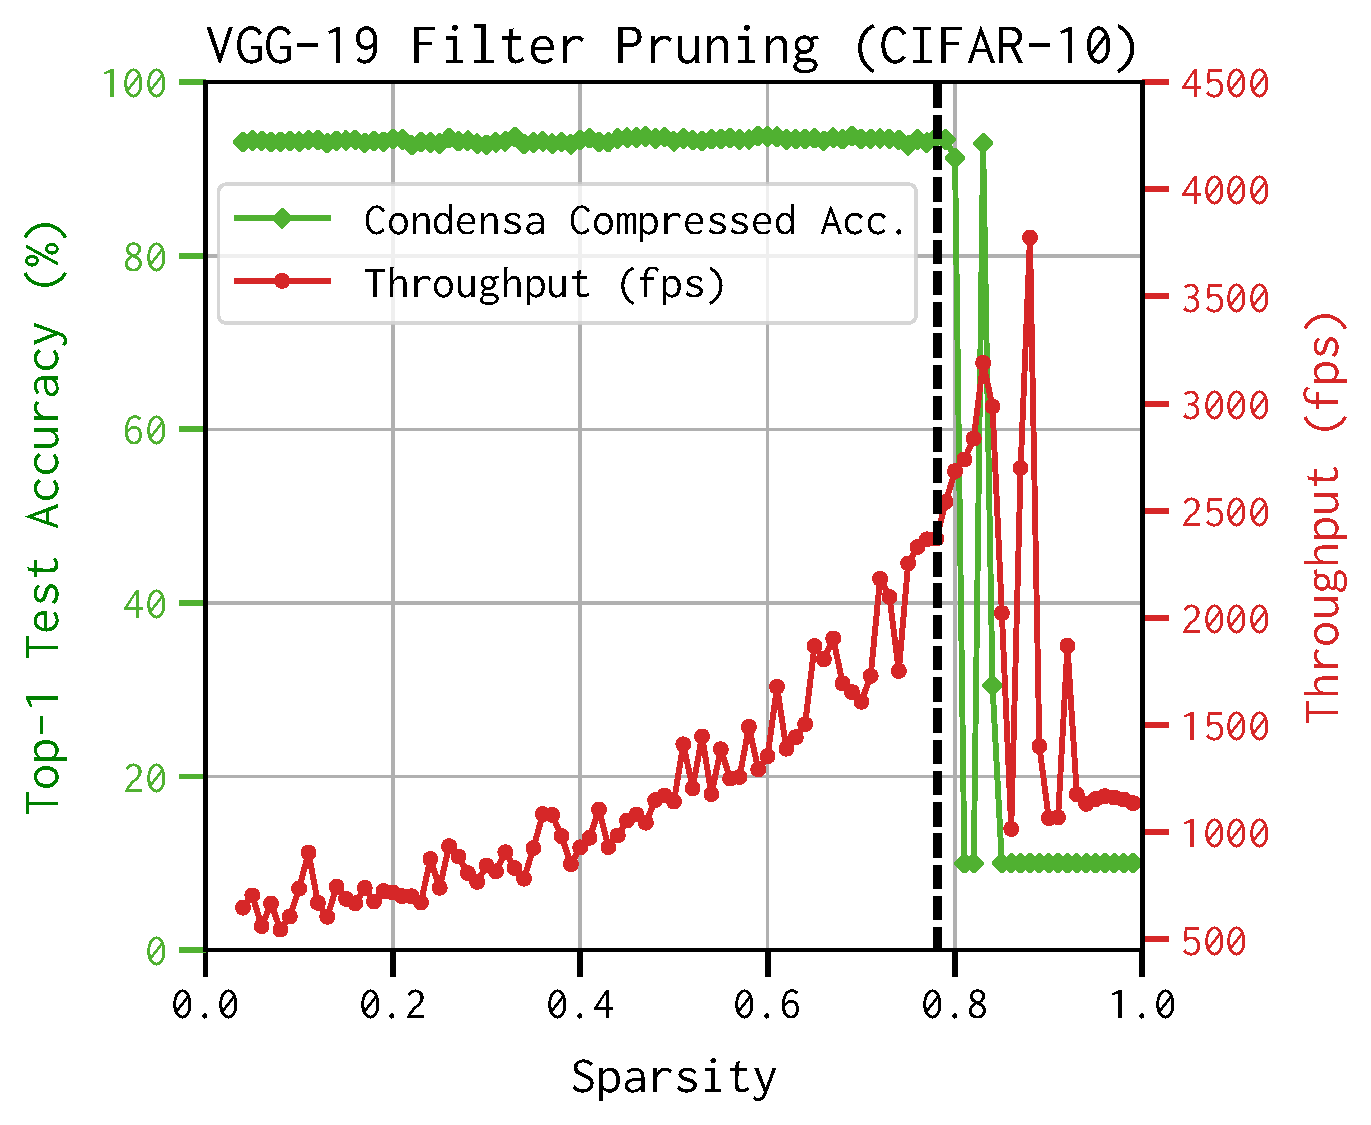
\includegraphics[width=0.5\linewidth]{img/vgg19_bn_filter_intro_v2.pdf}
%\vspace{-10pt}
\caption{Top-1 test accuracy (green) and throughput (red) vs.\ sparsity for VGG-19 on CIFAR-10.
\algoName is designed to solve constrained optimization problems of the form ``maximize throughput, with a lower bound on accuracy". In this case, \algoName automatically discovers a sparsity (vertical dashed line) and compresses the model to this sparsity,
improving throughput by $2.59\times$ and accuracy by $0.36\%$.
}
\vspace{-10pt}
\label{fig:vgg-intro}
\end{figure}

%Current approaches to model compression
%also require manual specification of compression hyperparameters, such
%as the target sparsity ratio, which is the proportion of zero-valued parameters in %the
%compressed model vs.\ the original.
%
Current approaches to model compression
also require manual specification of compression hyperparameters, such
as {\bf target sparsity}---{\em the proportion of zero-valued parameters in the
compressed model vs.\ the original.}
%
However, with current approaches, finding the best sparsity 
often becomes a trial-and-error search, with
each such trial having a huge cost (often multiple days for large models such as BERT) and involving training the compressed model to convergence,
only to find (in most cases) that the compression objectives are not met.
%
The main difficulty faced by such unguided approaches is
that sparsities 
vary unpredictably with changes in the compression context,
making it very difficult to provide users with any guidelines, whatsoever.
%
Therefore, automatic and {\em sample-efficient} approaches that minimize the number of trials are crucial
to support the needs of designers who must adapt
a variety of neural networks to a broad spectrum of platforms targeting a wide
range of tasks.

To address the above-mentioned problems of flexible expression of compression strategies, automated compression hyperparameter inference, and sample efficiency, we introduce \algoName, a new framework for programmable model compression. As an illustration of the level of automation provided by \algoName,
consider the problem of improving the
inference throughput of VGG-19~\cite{simonyan2014very} on the CIFAR-10 image
classification task~\cite{krizhevsky2014cifar}.
%
Since VGG-19 is a convolutional neural network, one way to improve its
inference performance on modern hardware such as GPUs is by pruning
away individual convolutional filters~\cite{he2018progressive}.
%
Figure~\ref{fig:vgg-intro} shows the accuracy and throughput obtained
by \algoName on this task.
%
Here, we plot the compressed model's top-1 test accuracy and throughput as a function of the sparsity (green and red lines,
respectively).\footnote{Note that these curves are not known a priori and
are often extremely expensive to sample;
they are only plotted here to better place the obtained solution in context.}
%
\algoName's solution corresponds to a sparsity of $0.79$
and is depicted as the vertical dashed line.
%
This result is significant for two reasons: (1) using the \algoName library,
the filter pruning strategy employed for this experiment was expressed in
less than 10 lines of Python code, and (2) the optimal sparsity of
$0.79$ that
achieves throughput and top-1 accuracy improvements of $2.59\times$ and $0.36\%$, respectively,
was obtained automatically by \algoName using a sample-efficient constrained
Bayesian optimization algorithm.
%
Here, the user didn't have to specify any
sparsities manually, and instead only had to define a domain-specific
objective function to maximize (inference throughput, in this case).





\begin{figure*}[!t]
\centering
  % \includegraphics[width=0.8\textwidth,height=10cm]{CVPR2021/img/FinalIntroFigure.pdf}
  \includegraphics[width=\textwidth]{img/FinalIntroFigure.pdf}
  \caption{Overview of our CIE reduction framework using label preservation-aware loss functions.}
  \label{fig:overview}
\end{figure*}

\end{refsection}
%\begin{refsection}

\section{Thesis Statement}
\label{sec:condensa}

%\end{refsection}
\begin{refsection}
\section{Research Work}
\label{sec:work}

\subsection{Condensa: A Programmable Approach to Neural Network Compression}
\subsubsection{Background, Related Work}

For a given task such as image classification, assume we have trained a large {\em reference} model $\overline{\bw} = \argmin_{\bw} L(\bw)$, where $L()$ denotes a {\em loss function} (e.g., cross-entropy on a given training set), and $\bw \in \mathbb{R}^P$. {\em Model compression} refers to finding a smaller model $\Theta$ that can be applied to the same task and ideally achieves the same accuracy as $\overline{\bw}$.
Model compression can be performed in various ways, and \algoName currently supports two commonly used techniques: pruning and quantization. In pruning, non-zero values from $\overline{\bw}$ are eliminated or ``pruned'' to obtain $\Theta$. Pruning is usually performed using some kind of thresholding (for eg., magnitude-based) and can be unstructured (prune any non-zero value) or structured (prune only {\em blocks} of non-zeros). On the other hand, quantization retains the number of parameters in $\Theta$ but assigns parameters in $\overline{\bw}$ one of K codebook values, where the codebook may be fixed or adaptive. \algoName supports low-precision approximation, which refers to assigning each parameter in $\overline{\bw}$ a corresponding lower-precision representation (for example, converting from 32-bit to 16-bit floating-point) and is equivalent to quantization using a fixed codebook.


\noindent \textbf{DNN Compression Techniques}
There is considerable prior work on accelerating neural networks using structured 
weight pruning~\cite{wang2019structured,mccarley2020structured,frankle2018lottery, han2015learning, luo2017thinet, han2017ese, dong2017more, han2016eie, polyak2015channel, hu2016network, anwar2016compact, molchanov2016pruning}, quantization~\cite{zhu2016trained, gong2014compressing} and 
low-rank tensor factorization~\cite{kossaifi2020factorized,lebedev2014speeding, xue2013restructuring, denton2014exploiting, girshick2015fast}.
Most of these individual compression
schemes for pruning and quantization and their combinations can be expressed in \algoName. Two common problems with these existing methods are: (1) determining optimal sparsity at a global (network) level, and (2) distributing global sparsity into per-layer sparsities.
We tackle these problems efficiently and systematically using our Bayesian and L-C optimizers, respectively, as described in Section~\ref{sec:condensa}.

\noindent \textbf{Automated Model Compression}
\begin{comment}
Bayesian optimization has previously been demonstrated to work well for general hyperparameter optimization in machine learning and neural architecture search~\cite{snoek2012practical,dai2019chamnet}.
To the best of our knowledge, we are the first to use sample-efficient search via Bayesian optimization for obtaining compression hyperparameters.
Automation in model compression is currently achieved either through reinforcement learning (RL) algorithms~\cite{he2018amc} or simulated annealing~\cite{liu2019autoslim}. 
In particular, the automation procedure for AMC~\cite{he2018amc} uses four arbitrary stages of pruning and re-training for RL training; additionally, the reward function is difficult to design, and even given a good reward, local optima can be hard to escape. It is also difficult to determine when such methods may just be overfitting to irrelevant patterns in the environment. Even disregarding generalization issues, AMC's agent (DDPG) uses trial and error, which is characterized to have an underlying incompatibility with the target pruning problem \cite{liu2019autoslim}.
AutoSlim~\cite{liu2019autoslim} proposes an automated approach based on simulated annealing, and uses the ADMM algorithm for accuracy recovery, which is an AL-based method very similar to the L-C algorithm; AutoSlim, however, only supports weight pruning and does not support general compression schemes as \algoName does. 
\end{comment}
Automating model compression involves finding both an optimal compression strategy for a given $\overline{\bw}$, along with its corresponding compression hyperparameters such as target sparsity with minimal manual intervention. Current state-of-the-art frameworks in this domain include AMC~\cite{he2018amc} and AutoCompress~\cite{liu2019autoslim}, which use reinforcement learning and simulated annealing, respectively, to automatically find desirable target sparsities for a fixed pruning strategy. \algoName, in contrast, supports the programmable expression of a wide variety of compression strategies (not just pruning). Also, in the context of automated model compression, each sample corresponds to training the compressed model to convergence, and can be extremely expensive to compute; unfortunately, techniques such as reinforcement learning, which is used in AMC~\cite{he2018amc}, can be highly sample-inefficient~\cite{mnih2013playing}. To minimize the number of samples drawn, \algoName uses a novel and sample-efficient Bayesian optimization-based algorithm for automatically arriving at desirable target sparsities. While Bayesian optimization has previously been demonstrated to work well for general hyperparameter optimization in machine learning and neural architecture search~\cite{snoek2012practical,dai2019chamnet}.
To the best of our knowledge, we are the first to use sample-efficient search via Bayesian optimization for obtaining compression hyperparameters.
%

\noindent \textbf{General Compression Algorithms and Tools} General accuracy recovery algorithms capable of handling a wide variety of compression techniques provide the foundation for systems like \algoName. Apart from the L-C algorithm~\cite{carreira2017model} which \algoName uses, other recent accuracy recovery algorithms have been proposed. ADAM-ADMM~\cite{zhang2018adam} proposes a unified framework for structured weight pruning based on ADMM that performs dynamic regularization in which the regularization target is updated in each iteration. DCP~\cite{zhuang2018discrimination} introduces additional losses into the network to increase the discriminative power of intermediate layers and select the most discriminative channels for each layer by considering the additional loss and the reconstruction error. \algoName can readily support such algorithms as additional optimizers as described in Section~\ref{sec:condensa}. Neural network distiller~\cite{neta_zmora_2018_1297430}, TensorFlow model optimization toolkit~\cite{tftoolkit} {\color{black} and NNCF~\cite{kozlov2020neural} are three recent open-source model compression frameworks that support multiple compression schemes.} While these projects share a number of common goals with \algoName, they differ in two important ways: first, they do not support the expression of schemes as imperative programs containing control-flow, iteration, recursion, etc.~(Distiller requires a declarative compression specification in YAML, while the TensorFlow model optimization toolkit operates by modifying the DNN computation graph directly); second, these frameworks do not support automatic compression hyperparameter optimization for black-box objective functions.

\subsubsection{Contribution}

This paper makes the following contributions:
\begin{enumerate}
    \item It presents \algoName, a new framework for programmable neural network compression. \algoName supports the expression of
the overall compression strategy in Python using operators provided by its compression library. 
%
Since each strategy is a Python function, users are  
able to programmatically compose elementary schemes to build much
more complex and practically interesting schemes.

\item It presents a novel sample-efficient algorithm based on Bayesian optimization (B.O.) in \algoName for automatically inferring optimal sparsities based on a user-provided objective function. Given \algoName's ability to support the expression of meaningful high-level
objective functions---for example, the throughput (images/sec) of a convolutional neural network---users
are freed from the burden of having to specify compression hyperparameters manually.

\item It demonstrates the effectiveness of \algoName on three image classification and language modeling tasks, resulting in memory footprint reductions of up to $188\times$ and runtime throughput improvements of up to $2.59\times$ using at most 10 samples per search.
\end{enumerate}
\subsection{Sample Efficient Methods for Compression Hyperparameter Search}
\subsubsection{Background, Related Work}
\subsubsection{Contribution}
\subsection{Correctness: Reliable Model Compression via Label-Preservation-Aware Loss Functions}
\subsubsection{Background, Related Work}

In this section, we provide a brief overview of recent model compression approaches, followed by a more detailed background on group sparsity-based model compression and CIE reduction.

% -- Upweighted CIEs (better way would be to only upweight CIEs which are not misclassified by the uncompressed model, but misclassified by the compressed model)
%
%\noindent \textbf{Model Compression}
%Definition
%LC-optimizers
%Rewind
%Magnitude-based
%Shortcomings of focusing on accuracy alone
\noindent \textbf{Model Compression}
Deep neural networks are heavy on computation and memory by design,
%
creating an impediment to operating these networks on resource-constrained platforms.
%
%
To alleviate this constraint, several branches of work 
have been proposed to reduce the size of an existing
neural network.
%
%
The most commonly employed approach 
is to reduce the number of weights, neurons, or layers in a 
network while maintaining approximately the same
performance~\cite{joseph2020programmable}.
%
This approach was first explored on DNNs
in early work such as~\cite{lecun1990optimal,hassibi1994optimal}.
%
%
Studies conducted by~\cite{han2015learning,han2015deep} %song han
showed that simple unstructured pruning can reduce the size
of the network by pruning unimportant connections within the 
network. However, such unstructured pruning strategies produce large sparse weight matrices that are computationally inefficient unless equipped with a specialized hardware~\cite{numenta20}.
%
%
To resolve this issue, structured pruning methods were proposed 
where entire channels are pruned simultaneously to ensure that the pruned network can be naturally accelerated on commodity hardware~\cite{li2016pruning,hu2016network,wen2016learning}. %the denseness of the weights.
%
More recently, Renda et al.~\cite{renda2020rewind} proposed the \textit{rewind} algorithm which is similar to simple fine-tuning of the network to regain the loss in accuracy incurred during the pruning step. The sparsity level of the model is updated in small steps where each step enhances the sparsity of the model followed by fine-tuning.
The two major schemes for structured pruning are either based on filter pruning~\cite{joseph2019condensa} or low-rank tensor factorization~\cite{li2020group}. Both these approaches enable direct acceleration of the networks in contrast to unstructured pruning.
Li et al.~\cite{li2020group} explored the relationship between tensor factorization and general pruning methods, and proposed a unified approach based on sparsity-inducing norm which can be interpreted as both tensor factorization or direct filter pruning. By simply changing the way the sparsity regularization is enforced, filter pruning and low-rank decomposition can be derived accordingly. 
This is particularly important for the compression of popular network architectures with shortcut connections (e.g. ResNet), where filter pruning cannot deal with the last convolutional layer in a ResBlock while the low-rank decomposition methods can.

\paragraph{Accuracy Recovery Algorithms} General accuracy recovery algorithms capable of handling a wide variety of compression techniques provide the foundation for modern compression systems. Prior work in this domain includes the LC algorithm~\cite{carreira2017model}, ADAM-ADMM~\cite{zhang2018adam} and DCP~\cite{zhuang2018discrimination}. More recently,
%like \algoName. Apart from the L-C algorithm~\cite{carreira2017model} which \algoName uses, other accuracy recovery algorithms are also suitable for our \emph{label-preservation loss function} formulation, for example ADAM-ADMM~\cite{zhang2018adam} a unified framework for structured weight pruning based on ADMM that performs dynamic regularization in which the regularization target is updated in each iteration.
%and also DCP~\cite{zhuang2018discrimination} which has additional losses into the network to increase the discriminative power of intermediate layers and select the most discriminative channels for each layer by considering the additional loss and the reconstruction error. 
the \textit{Rewind}~\cite{renda2020rewind} and Group-Sparsity~\cite{li2020group} algorithms have been demonstrated to be state-of-the-art compression algorithms.
Due to their compression scheme-agnostic nature, we build upon these two methods in our paper to evaluate the proposed \emph{label-preservation-aware loss functions} as described in Section~\ref{sec:losses}.
%Both these formulations are independent of both the compression scheme ($\mathcal{H}$) and the compression accuracy recovery algorithm ($\mathcal{A}$) itself given that the method allows optimizing over arbitrary differentiable loss functions.
%

\paragraph{Network Distillation}
%Teacher-student learning?
%Logit Pairing
%Kannan et al. (2018)~\cite{kannan2018adversariallogit} used the idea of logit pairing between different images to .
%Knowledge distillation (Hinton)
Another branch of network compression initially proposed by \cite{hinton2015distilling}, attempts to distill knowledge from a large teacher network to a small student network. 
%attempts to reduce the size of the network by transferring the knowledge of the full network to a student network of smaller size.
%
% By employing a loss function that teaches the student network to mimic the outputs of the teacher network, a smaller network with similar performance can be obtained.
With the assumption that the knowledge captured by a network is reflected in the output probability distribution, this line of work trains the student network to mimic the probability distribution produced by the teacher network. Since the networks are trained to output one-hot distribution, a temperature $T$ is used to diffuse the probability mass.
%
Advanced methods of distillation have succeeded in achieving much more effective transfer by not only
transferring the output logits but the information of the intermediate activations as in~\cite{zagoruyko2016paying, romero2014fitnets, jang2019learning, ahn2019variational}.
Although network distillation was presented as a general form of logit pairing, it is quite difficult to obtain improvements during distillation without spending considerable effort in manually tuning the temperature $T$ for the softmax layer. In contrast, using pure logit pairing comes without any additional cost of manual hyperparameter tuning.
Therefore, we employ pure logit pairing instead of knowledge distillation in our approach.


%
% loss function learning
% ref https://arxiv.org/pdf/1912.12355.pdf
% SoftAdapt: Techniques for Adaptive Loss Weighting of 
% Neural Networks with Multi-Part Loss Functions
%

\paragraph{Group-Sparsity based Model Compression}
%\label{sec:group_sparsity}

We now briefly describe the key insight of the compression recovery algorithm that was used in our evaluation.
The main idea in the Group-Sparsity recovery algorithm \cite{li2020group} is that the filter pruning and filter decomposition seek a compact
approximation of the parameter tensors despite their different operational forms to cope with different application scenarios.
%
Consider a vectorized image patch  $\bf{x} \in \mathbb{R}^{m \times 1}$
and a group of $n$ filters $\bf{\mathcal{W}} = \{\bf{w_1}, \cdots , \bf{w_n}\} \in \mathbb{R}^{m \times n}$.
%
The pruning methods remove output channels and approximate the original output $\bf{x}^T \bf{\mathcal{W}}$ as $\bf{x}^T \bf{C}$, where $\bf{C} \in \mathbb{R}^{m \times k}$ only has
$k$ output channels. Filter decomposition methods approximate $\bf{\mathcal{W}}$ as two filters $\bf{A} \in \mathbb{R}^{m\times k}$
and $\bf{B} \in \mathbb{R}^{k \times n}$, making $\bf{AB}$
a rank $k$ approximation of $\bf{\mathcal{W}}$. 
%
Thus, both pruning and decomposition-based methods seek a compact approximation to the original network parameters, but adopt different strategies for the approximation.
%
%
The weight parameters $\bf{\mathcal{W}}$ are usually trained with some regularization 
such as weight decay to constrain the hypothesis class.
%
To get structured pruning of the filter, structured sparsity regularization 
is used to constrain the filter:
\begin{equation}
\min _{\mathcal{W}} \mathcal{L}(y, \Phi(\mathbf{x} ; \mathcal{W}))+\mu \mathcal{D}(\mathcal{W})+\lambda \mathcal{R}(\mathcal{W})
\label{eq:loss1}
\end{equation}
%
where $\mathcal{D}(\cdot)$ and $\mathcal{R}(\cdot)$ represents the weight decay and 
sparsity regularization term respectively, while $\mu$ and $\lambda$ are the regularization factors.
%
Instead of directly regularizing the matrix $\bf{\mathcal{W}}$ \cite{yoon2017combined, li2019oicsr}, we enforced group sparsity constraints by incorporating a sparsity-inducing matrix $\mathbf{A} \in \mathbb{R}^{n \times n}$, which can be converted to the filter of a $1 \times 1$ convolution layer after the original layer.
%
%
Then the original convolution of 
$Z = X \times \mathcal{W}$ becomes 
$Z = X \times (\mathcal{W} \times \mathbf{A})$.
%
To obtain a structured sparse matrix, group sparsity regularization is enforced on $\bf{A}$. Thus, the loss Eqn. \ref{eq:loss1} function becomes
%
\begin{equation}
\min _{\mathcal{W}, \mathbf{A}} \mathcal{L}(y, \Phi(\mathbf{x} ; \mathcal{W}, \mathbf{A}))+\mu \mathcal{D}(\mathcal{W})+\lambda \mathcal{R}(\mathbf{A})
\label{eq:loss2}
\end{equation}
%
Solving the problem in Eqn. \ref{eq:loss2} results in structured group
sparsity in matrix $\textbf{A}$. By considering matrix $\bf{\mathcal{W}}$ and $\bf{A}$ together, the actual effect is that the original convolutional
filter is compressed.

\paragraph{Compression Impacted Exemplars (CIEs)}

Top-1 accuracy is just one among many possible ways of characterizing the quality of a compressed model. An alternative approach involves counting all the inputs for which the compressed model disagrees with the original, uncompressed model. Each such input is termed a {\em Compression Impacted Exemplar (CIE)}, following the definition by Hooker et al.~\cite{hooker2020characterising} (see also footnote~\ref{footnote:cie-cie}). %\sscmt{But Sara's definition was Compression Identified Exemplar. I think we should mention this explicitly without just saying that we follow the definition of Hooker et al. since this slightly deviates from it.}
While CIE reduction is critical in domains which require compressed models to match the original model as closely as possible,
we observe that reducing label mismatches is all the more important {\em when the reference model makes a correct prediction}. We term such CIEs {\em CIE-U}. In Section~\ref{sec:losses}, we explore novel loss formulations that target both CIE and CIE-U reduction during compression.

%we observe that CIEs can be of two kinds, each with very different characteristics:

%\begin{itemize}
%    \item \textbf{CIE-C:} A CIE which the compressed model gets right (w.r.t. ground truth) but the uncompressed model gets wrong.
%    \item \textbf{CIE-U:} A CIE which the uncompressed model gets right (w.r.t. ground truth) but the compressed model gets wrong.
%\end{itemize}

%While reducing both types of CIEs is desirable for cases where the compressed model must match the reference model as closely as possible, note that there may be domains which care more about reducing CIE-Us alone (i.e., if the reference model makes a correct prediction, ensure that the compressed one does too). In Section~\ref{sec:losses}, we explore novel loss formulations to reduce the different types of CIEs subject to such constraints.
%We notice that reducing the number of CIE-Cs can {\em hamper} the performance of the final model, and that an effective CIE reduction algorithm must focus on reducing CIE-Us instead.

CIE reduction has received relatively little attention from the research community, with recent work by Hooker et al.~\cite{hooker2020characterising} being the only one that we are aware of that tries to identify and reduce CIEs. Their primary approach  involves re-weighting CIEs, where they consider a mitigation strategy of fine-tuning the compressed model for a certain number (chosen to be 3000) of iterations while up-weighting the CIEs relative
to the rest of the dataset. Their approach is sensitive to hyperparameters such as: (1) choice of number of fine-tuning iterations, (2) a threshold (90th percentile) to upweight all exemplars above that threshold, and (3) an upweighting value of $\lambda > 1$ for CIE which they choose to be $2$. We believe that our approach  is more principled for a number of reasons. First, we pose CIE mitigation as a general \emph{label-preservation} problem and extensively explore several loss functions to mitigate this without introducing any new hyperparameters than were initially used during model compression or changing any of the values of the original compression hyperparameters. Lastly, we are agnostic to the compression scheme and compression algorithm.

%In Section~\ref{sec:losses}, we introduce novel loss functions that are specifically designed to reduce total CIEs and CIE-Us without adversely affecting CIE-Cs. 
%\noindent Minimizing the disagreement between the two models in the first case will hamper it's performance on the data, which is undesirable. Therefore, minimization only in the second case is desirable. In order to circumvent this problem, we again introduce the cross-entropy loss into the picture, but in conjunction with the logit pairing loss.




\paragraph{Multi-Part Loss Functions} 
% soft-adapt
% Recently more work is being done on how loss functions affect learning 
Networks that perform challenging tasks or multiple 
tasks often require a combination of losses to work. Considerable effort has been made towards understanding the role of different loss terms~\cite{huang2019addressing,barron2019general,chen2018gradnorm}, and how best to combine them. 
%
%
% Multiple losses are typically combined by taking an 
% equally-weighted linear combination of
% each objective function; but the importance of each part
% could be different and thus components should be assigned...
% weights as per their contribution to the learning. 
While most of the prior work combines these losses either using ad-hoc or equal weights, %. However, the actual contribution of each loss is difficult to manually compute. The weights of different loss functions can even vary over the training time where some losses can be useful to initially bootstrap the model while some are useful in gaining an extra performance boost towards the end of the training cycle.
%
% On the other hand, the scaling of each component of the 
% loss function can inhibit the ability of the optimizer 
% by only looking at loss components with the largest magnitude.
% ...
%In recent years, the need for weighting the components
%of multi-part functions has become more evident, and 
researchers have recently tried to develop systematic methods to adjust
the weights on the linear combination of loss components.
%
%
These methods often require defining new loss functions~\cite{barron2019general} or changing the optimization procedure~\cite{chen2018gradnorm}. %, but there is limited research on the formulation of a general method
%that can be added to existing architectures. 
%
%
%In most cases, the integration with the current models requires sophisticated adjustment or much longer computation time.
As we describe in Section~\ref{sec:loss_opti}, we compare three different hyperparameter tuning strategies to optimize our multi-part loss function.

\subsubsection{Contribution}

\noindent Our key contributions in this work are as follows:
\begin{itemize}
    \item Employing additional loss terms in the compression objective based on the teacher-student paradigm so as to align the predictions of the reference and the compressed models. %logit pairing term into the network compression objective, thus exploiting the teacher-student learning paradigm along with a term for aligning the predictions of the reference and compressed models. \sscmt{Both of these are the same. Do you mean aligning predictions of the compressed model and the actual targets?} 
    We show for the first time that such a pairing can be extended to other tasks, by considering semantic segmentation. Figure~\ref{fig:motivation} shows an example of the effect of the different loss terms on the number of model mismatches.
    \item Analyzing automated strategies for tuning the hyperparameters associated with our multi-part loss functions. We demonstrate that our framework is robust to the choice of tuning strategies, and uniform weighting works as well as more intricate strategies across different datasets and reference network architectures.
    \item Through extensive experiments, we validate the effectiveness of our framework and show that it not only improves metrics such as the number of CIEs, but also yields better compression accuracy compared to previous approaches. %\sscmt{perhaps we should mention that it's mainly due to the fact that we further decompose CIEs into CIEs-U and CIEs-C, and optimize not to align the logits in cases where the prediction of the reference model is wrong}. 
\end{itemize}

% What is a good way to design a label-preservation optimization formulation
% Trying to be Agnostic to Compression Recovery Algorithms.

While the teacher-student paradigm is a coarse way to capture ``semantic similarity'' between the reference and compressed models, our results show that it can nonetheless be highly effective in reducing the number of CIEs.
We also remark that our methodology can work with any compression scheme that allows us to specify a custom objective that can be optimized to produce a compressed model. 
\subsection{Proposed Work}

\subsubsection{Class-wise CIEs: Mitigating The Bias problem for Fairness in Edge Inference}

\subsubsection{Attribution Matching for Sensitive Edge Inference Tasks}

Mitigating the impact of compression is particularly
urgent given the widespread use of compressed deep 
neural networks in resource constrained but sensitive 
domains such as 
%
%
%
health care diagnostics 
\cite{xie2019automated, %(Xie et al., 2019; 
gruetzemacher20183d,    %Gruetzemacher et al., 2018; 
badgeley2019deep,       %$Badgeley et al., 2019;
oakden2020hidden}       %Oakden-Rayner et al., 2019),
%
%
,self-driving cars 
\cite{teslacrash17} %(NHTSA, 2017)
%
facial recognition software
\cite{
buolamwini2018gender% Buolamwini
 % Gebru, 2018b). 
} and
%
hiring
\cite{amazon18, 
yourface19}.% Harwell2019
%
%
For these tasks, the trade-offs incurred by 
compression will be intolerable given the huge impact 
on human welfare.
%
\cmt{Due to the success of Deep learning, there is an 
emergent trend to utilize deep neural networks (DNNs) 
even for safety-critical applications such as 
self-driving cars and health-care applications 
\cite{estava2017dermatologist,
samala2018evolutionary, lane2018deep}}.
%
Due to the inherent nature of such devices, 
it is of paramount importance that the utilized 
DNNs be reliable and trustworthy to human users.
%

For a system to be reliable, perpetual service 
must be rendered and the integrity of the system 
must hold even under unexpected circumstances.
%
%
For most commercially deployed DNNs, this condition 
is hardly met as they are often operated in the 
cloud due to their heavy computational requirements.
%
%
However, this dependence on clouds acts as a 
critical weakness in safety-sensitive settings 
as intermittent communication failuers to the 
cloud may cause difficulties in reacting to 
situations immediately, or even-worse, 
the device's connection to the cloud may be 
severed indefinitely.
%
%
Thus, to guarantee reliable service, 
the DNNs must be embedded on the edge device.
%
%
%
To this end, network compression techniques such 
as pruning \cite{han2015deep,li2016pruning} and distillation \cite{hinton2015distilling,zagoruyko2016paying} 
are commonly employed - as a compressed network 
would require less computational time and memory 
but maintain its prediction performance to a 
certain acceptable margin, effectively substituting 
the original network for edge computation.

\vcmt{This text is for attribution-perservation, we need to rewrite for label-preservation}
\cmt{At the same time, for a system to be trustworthy, 
the system must be transparent enough for humans 
to understand its workings and the reasons for its outputs.
%
%
An example would be when a health monitor 
predicts an onset of disease \cite{xu2019current}
- then the clinician would require an acceptable
explanation to the device output.
%
%
However, the black-box nature of deep neural 
networks complicates this goal - impeding its 
advance in safety-critical areas.
%
%
For DNNs to gain trustworthiness, the ability 
to explain why the network makes such decisions 
is essential. Such field of interest - 
eXplainable AI (XAI) - has emerged as one of the 
importance frontiers in the field of deep learning.
%
%
Amoung numerous XAI methods, the most commonly 
used methods are attribution methods \cite{selvaraju2017grad}, 
which weigh the parts of the input data according to 
how much they 'contributed' to produce the output prediction.
%
%
Such attribution methods are beginning to be applied
in safety-critical fields \cite{liang2020prediction}.}

To ensure the safety of the system, 
the two aforementioned conditions should be simultaneously 
satisfied - the embedded DNNs must be equipped with 
both compression and attribution.
%
%
However we show for the first time that these seemingly
unrelated techniques conflict with each other:
\vcmt{compressing a network causes deformations in 
the produced attributions, even if the predictions 
of the network stays the same before and after compression.}
%
%
\vcmt{This is a potentially severe crack in the 
integrity of the compressed network, 
as the premise in which a compressed network 
is acceptable in safety-critical fields is that 
the compressed network in as reliable as its former self}.
%
%
\textit{This implies that the compressed nework must behave 
almost identically to the pre-compression network while being
smaller in size.}
%
%
Moreover, the classifications between the network are
not only different from their past counterparts 
but also broken down compared to their respective ground truths
%
%
\begin{itemize}
    \item Examples where the compressed model gets the example 
          right but the uncompressed model gets it wrong.
    \item Examples where the uncompressed model gets it right 
          but the compressed model gets it wrong.
\end{itemize}
%
%
These label distortions directly
cause incorrect interpretations, which could lead to dire 
consequences for safety-critical systems.
%
%
Such a problem arises from the pitfall of existing 
network compression approaches: they only
aim to maintain the prediction quality of the network while 
reducing the size of the network.
%
%
Compressing a network forces the network to cram its 
necessary decision procedures and information inside a
smaller space.
%
This space restriction forces the network to abandon its 
standard decision procedures and resort to using shortcuts 
and hints that are seemingly indecipherable to humans.
%
Thus, its decision procedures would become harder to 
interpret, which is reflected in its production of deformed
attribution maps
%
%
To resolve this newfound unintended
issue, we propose a novel label-preservation aware 
compression framework  to ensure both the reliability and 
trustworthiness of the compressed model.
%
...we concentrate on the observation that the labels 
of the pre-network (teacher) are closer to the ground truth signal 
compared to the post-network (student).
%
Thus, in the absence of ground truth signals, the labels
of the teacher can serve as a proxy. 
%
In this sense, we propose a automatically parameter 
tuned regularizer learning framework that matches the 
of the now-compressing network to its attribution maps 
before compression, transferring the attributional power 
of the pre-network to the post-network. Our work sheds 
new light on transfer learning techniques from the perspective of XAI,
as they can be re-interpreted and subsumed under our framework.



\end{refsection}
%\begin{refsection}
\section{Timeline, Remaining Work, Plans}
\label{sec:timeline}

\begin{table*}[h]
\centering
\begin{center}
%\begin{scriptsize}
\begin{sc}
\begin{tabular}{ll}
\toprule
\textbf{Papers, Patents and Presentations}                                                  & \textbf{Timeline}        \\ \midrule
Effective Paralleization of Belief Propation on the GPU                  & NVIDIA GTC 2018          \\ 
Message scheduling for performant, many-core belief propagation.         & IEEE HPEC 2019           \\ \midrule
A Programming System and Automation Libraries for Model Compression                           & Baylearn-19, NeurIPS-19, GTC-19 \\
Model Compression for Health care Devices Challenges and Opportunities    & GE HealthCare 2019       \\
A Programmable Approach for Neural Network  Compression                  & IEEE MICRO 2020          \\
Bayesian Optimization for Model Compression                              & NVIDIA 2019              \\ \midrule
Correctness-preserving Compression of Datasets and Neural Networks & Correctness SC 2020      \\
Reliable Model Compression via Label-Preservation-Aware Loss Functions   & CVPR 2020 (Under Review) \\
Mitigating the Bias \& Attribution Problems for Safety \& Fairness & KDD 2021 (Proposed Venue)                             \\ \midrule
\textbf{Dissertation Defense}                                            & \textbf{Spring 2021} \\   
\bottomrule
\end{tabular}
\label{tab:results}
  \end{sc}
%\end{scriptsize}
\end{center}
\end{table*}

%\end{refsection}
%%\begin{refsection}
\section{Broader Impact} 

Non-Vision Apps

Scene-Graph Preservation

Condensa-ZFP : Using New Loss functions

%\end{refsection}
\printbibliography

\end{document}

%%% Local Variables:
%%% mode: latex
%%% TeX-master: "root"
%%% End:
